\documentclass[conference,a4paper]{IEEEtran}
% ICCIT 2026 requires an anonymous initial manuscript. Add the author block only
% after acceptance, when preparing the camera-ready version.

\usepackage{cite}
\usepackage{amsmath,amssymb,amsfonts}
\usepackage{graphicx}
\usepackage{textcomp}
\usepackage{xcolor}
\usepackage{booktabs}
\usepackage{tikz}
\usepackage{url}
\usetikzlibrary{arrows.meta,calc,fit,positioning}
\urlstyle{same}

\definecolor{jbblue}{RGB}{32,86,130}
\definecolor{jbteal}{RGB}{25,112,105}
\definecolor{jbamber}{RGB}{168,105,28}
\definecolor{jbred}{RGB}{157,45,45}
\definecolor{jbgray}{RGB}{242,244,246}

\def\BibTeX{{\rm B\kern-.05em{\sc i\kern-.025em b}\kern-.08em
    T\kern-.1667em\lower.7ex\hbox{E}\kern-.125emX}}

\begin{document}

\title{Partition-Resilient Federation Across Simulated ISP Islands}

\author{}

\maketitle
\vspace{-1.5\baselineskip}

\begin{abstract}
Federated services retain local availability during a network partition, but cross-instance
communication stops when instances cannot route to one another. External-relay circumvention also
requires a path beyond the isolated region. This paper studies the narrower condition in which some
domestic IP components survive while international transit or inter-ISP reachability does not. We
implement a public discussion service that exchanges content-derived, author-signed objects over
surviving paths. Nodes without inbound reachability synchronize in both directions through
outbound-initiated delivery and backfill. A configured multi-homed node binds connections to the
correct uplink and relays only after normal object validation. In a four-node container testbed, 19
topology, source-binding, relay, quota, and failover checks passed. After removal of the simulated
exchange, the three objects needed to render a new post reached the remote island in 0.5, 1.2, and
2.1 s in a controlled run. An earlier serial, deadline-free outbox stalled the same crossing for
407.6 s behind one blackholed peer. Concurrent per-peer draining removed this dependency. In a
separate eight-node chain, all 200 paced posts reached hop seven, with 4.125 s median and 6.115 s
99th-percentile latency. These results demonstrate mechanism feasibility under controlled
partitions. They do not establish that usable domestic paths survive a real shutdown.
\end{abstract}

\begin{IEEEkeywords}
federated systems, Internet shutdowns, network partitions, multi-homing, store-and-forward
\end{IEEEkeywords}

\section{Introduction}

Internet shutdowns remove different forms of reachability at different times. Measurement studies
distinguish deliberate shutdowns from faults and show that disruptions vary in scope and mechanism
\cite{bischof2023shutdowns}. During the July 2024 disruption in Bangladesh, measurement platforms
observed filtering, throttling, and a near-countrywide loss of Internet connectivity
\cite{ooni2025bangladesh}. Those observations establish the disruption, but they do not establish
that ordinary users on different domestic Internet service providers (ISPs) remained mutually
routable. We therefore treat surviving domestic connectivity as a deployment condition, not as a
claim about that event.

This distinction exposes a systems question. A conventional federated server can continue serving
local state during a partition, yet remote delivery requires a route to the other server. The
ActivityPub model, for example, normally delivers an activity by posting it to a remote actor's inbox
URL \cite{activitypub}. External-relay circumvention systems solve a different problem. Telex places
friendly infrastructure on paths to uncensored destinations \cite{wustrow2011telex}, while
Snowflake forwards through temporary proxies toward a centralized Tor bridge
\cite{bocovich2024snowflake}. These designs are useful while an external path exists. They do not
define server federation between domestic components that cannot reach that infrastructure.

We examine a conditional goal: preserve public discussion within each surviving IP component,
continue federation across any route that remains, and cross isolated ISP components when an
explicitly configured node has a usable uplink into each. The prototype is a forum rather than a
messaging overlay, so content must remain addressable, deduplicable, and verifiable after replication.

This paper makes three contributions.

\begin{itemize}
  \item It defines a reachability model for federated services and implements bidirectional
  synchronization for nodes that advertise no inbound endpoint.
  \item It implements a source-bound, multi-homed bridge that applies the same content validation as
  an ordinary receiver. Peer trust controls volume, not validity.
  \item It evaluates the composition under controlled route removal and multi-hop propagation. The
  evaluation includes a deployed failure in which one blackholed peer blocked every reachable peer,
  and the per-peer concurrency rule derived from that failure.
\end{itemize}

The result is not a general claim of censorship resistance. The system requires at least one
surviving path, does not conceal traffic metadata, and has not been deployed across independent
commercial ISPs during a shutdown.

\section{Related Work}

\textbf{Shutdowns and circumvention:} Bischof \emph{et al.} combine routing measurements, operator
statistics, and event data to characterize shutdowns and outages \cite{bischof2023shutdowns}. OONI's
Bangladesh report provides the event-specific measurement basis used here
\cite{ooni2025bangladesh}. Telex and Snowflake increase the censor's blocking cost through external
infrastructure and address churn, respectively \cite{wustrow2011telex,bocovich2024snowflake}. Our
system does not replace these tools. It targets the case where their external destination is
unreachable but some domestic paths remain.

\textbf{Decentralized publication and federation:} ActivityPub specifies interoperable
server-to-server social delivery \cite{activitypub}. Its endpoint-oriented model does not itself
restore a route between disconnected server components. Empirical work on Mastodon also shows that
software decentralization does not remove infrastructure concentration. In the measured graph of
Raman \emph{et al.}, removing instances in five autonomous systems reduced the largest connected
component from 92\% to 46\% of users \cite{raman2019mastodon}. Secure Scuttlebutt (SSB) is closer to
our object model: it uses signed author feeds and supports intermittent social replication
\cite{tarr2019ssb}. SSB emphasizes peer replication and subjective application state. We retain
independently operated servers, server-side projections, local moderation, scoped endpoints, and an
explicit multi-ISP relay policy.

\textbf{Disruption tolerance and multiple paths:} Bundle Protocol version 7 provides
store-and-forward delivery across intermittently connected networks \cite{rfc9171}. The durable
outbox and backfill mechanisms in our design apply the same general principle to federated
application objects. Interactive Connectivity Establishment and Multipath TCP maintain and rank
candidate paths \cite{rfc8445,rfc8684}. We rank paths by operational reachability scope and bind
outgoing sockets to an ISP-specific source address. This is an application-level availability
policy, not a new transport protocol.

\section{Reachability and Adversary Model}

Fig.~\ref{fig:model} defines four reachability states. R0 is ordinary global reach. At R1,
international transit is unavailable but a domestic route between participating nodes remains. At
R2, inter-ISP reachability is also absent, leaving disjoint components. R3 denotes an R2 topology in
which a multi-homed node retains one usable route into each component and is authorized to relay.
R3 is therefore a restoration mechanism, not a lower network layer. If every access link is cut,
the system can continue locally and queue work, but it cannot deliver across components.

\begin{figure}[t]
\centering
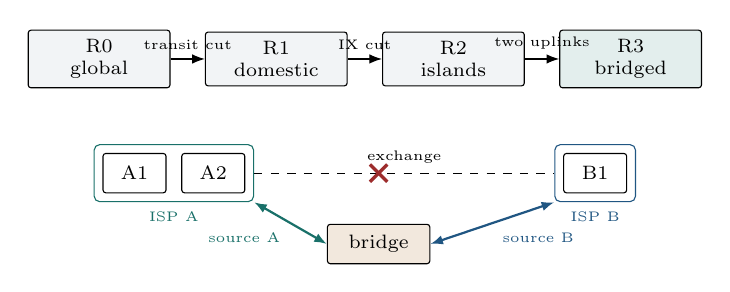
\begin{tikzpicture}[
  font=\scriptsize,
  rung/.style={draw,rounded corners=1pt,minimum width=18mm,minimum height=5.5mm,
               align=center,fill=jbgray},
  node/.style={draw,rounded corners=1pt,minimum width=8mm,minimum height=5mm,fill=white},
  island/.style={draw,rounded corners=2pt,inner sep=3pt},
  >={Latex[length=1.6mm]}
]
  \node[rung] (r0) at (0,0) {R0\\global};
  \node[rung] (r1) at (2.25,0) {R1\\domestic};
  \node[rung] (r2) at (4.50,0) {R2\\islands};
  \node[rung,fill=jbteal!12] (r3) at (6.75,0) {R3\\bridged};
  \draw[->] (r0) -- node[above,font=\tiny]{transit cut} (r1);
  \draw[->] (r1) -- node[above,font=\tiny]{IX cut} (r2);
  \draw[->] (r2) -- node[above,font=\tiny]{two uplinks} (r3);

  \node[node] (a1) at (0.45,-1.45) {A1};
  \node[node] (a2) at (1.45,-1.45) {A2};
  \node[island,fit=(a1)(a2),draw=jbteal,label={[font=\tiny,text=jbteal]below:ISP A}] (ia) {};
  \node[node] (b1) at (6.30,-1.45) {B1};
  \node[island,fit=(b1),draw=jbblue,label={[font=\tiny,text=jbblue]below:ISP B}] (ib) {};
  \node[node,fill=jbamber!15,minimum width=13mm] (br) at (3.55,-2.35) {bridge};
  \draw[<->,thick,jbteal] (ia.south east) -- node[below left,font=\tiny]{source A} (br.west);
  \draw[<->,thick,jbblue] (br.east) -- node[below right,font=\tiny]{source B} (ib.south west);
  \draw[dashed] (ia.east) -- node[above,font=\tiny]{exchange} (ib.west);
  \coordinate (cut) at (3.55,-1.45);
  \draw[jbred,very thick] ($(cut)+(-0.11,-0.11)$) -- ($(cut)+(0.11,0.11)$);
  \draw[jbred,very thick] ($(cut)+(-0.11,0.11)$) -- ($(cut)+(0.11,-0.11)$);
\end{tikzpicture}
\caption{Reachability states and the R3 test topology. After the simulated exchange is removed, the
multi-homed node is the only application path between ISP A and ISP B.}
\label{fig:model}
\end{figure}

The network adversary may remove or blackhole routes, block DNS names or IP addresses, throttle
connections, observe timing and volume on links it controls, and operate a federated peer. We assume
it cannot break Ed25519 \cite{bernstein2012ed25519} or SHA-256, extract an uncompromised endpoint
key, or control all discovered peers and bridges. We do not claim resistance to traffic correlation,
endpoint compromise, bridge coercion, eclipse attacks, power loss, or a total physical
disconnection.

\section{System Design}

\subsection{Self-authenticating application objects}

Every write is an envelope containing a version, domain, identity plane, author key, timestamp,
priority, opaque body, and signature. Let $C(E)$ be the restricted canonical encoding of the signed
fields of envelope $E$. The identifier and signature are
\begin{equation}
\begin{aligned}
  \mathit{id}(E)&=\operatorname{B32}\!\left(\operatorname{SHA256}(C(E))\right),\\
  \sigma&=\operatorname{Ed25519.Sign}_{sk}(C(E)).
\end{aligned}
\end{equation}
Protobuf serialization is not canonical across implementations or builds
\cite{protobufcanonical}. The receiver therefore parses, re-encodes under the restricted profile,
and rejects a byte mismatch. It verifies the signature against the bytes that arrived rather than a
repaired representation. The accepted profile uses ordered fields, omits default values, rejects
unknown fields, normalizes strings to NFC, and excludes floating-point fields from signed objects.
This is a correctness invariant, not a novelty claim. TypeScript, Rust, and Python implementations
agree byte-for-byte on 16 conformance vectors. The small vector set checks specified edge cases but
does not replace differential fuzzing.

Local and federated envelopes enter the same validation sequence:
\begin{equation}
\begin{aligned}
\text{parse/crypto}&\rightarrow\text{semantic admission}\\
&\rightarrow\text{atomic projection+witness}\rightarrow\text{fanout}.
\end{aligned}
\end{equation}
A trusted peer receives higher quotas and more traffic classes, but no signature, canonicality,
replay, or authorization check is skipped. Local user submissions pay an origin-specific cost through
proof of work, credits, or anonymous credentials. A remote node cannot verify that an independently
controlled origin actually charged that cost. Federated protection is therefore stated separately:
local submission is priced, while a malicious origin is bounded by receiver-side per-peer and
per-class quotas.

\subsection{Outbound-only bidirectional federation}

The sending path writes one durable outbox row per eligible peer and retries with backoff. The
receiving path records a monotonic stream position and requests missing objects after reconnection.
A node may advertise no endpoint. It still sends queued objects over a connection it opens and
receives remote objects by opening a connection and requesting backfill. Thus, both directions are
initiated by the node behind carrier-grade network address translation (CGNAT). Unique constraints on
$(\mathit{content\_id},\mathit{direction})$ make overlapping live delivery and backfill idempotent.
An object is never fanned back to the peer from which it arrived.

\subsection{Source-bound bridging}

Each endpoint is labeled with a reachability scope, autonomous system number, and eligible uplink.
Active probes maintain the live scope of each uplink. A node prefers the narrowest usable path so an
ISP-local route stays active while broader reach fails. For a remote island, the transport binds the
outgoing socket to the configured local address on the matching uplink. Relying on the host's default
route is insufficient: the peer may have no return route to the selected source.

The bridge is an ordinary validating node with a relay policy. It may relay an envelope only when
the origin peer and a target peer resolve to different uplinks and the bridge has trusted peers on
both sides. It charges one quota per uplink pair, not once per target peer. Bulk traffic is capped at
half of the pair's allocation so high-priority classes retain capacity. The bridge cannot alter a
signed object or admit an invalid one. It can still omit, delay, observe, or refuse traffic.

\subsection{Failure isolation and log observations}

Outbox entries are grouped by peer and identity plane. Groups are drained concurrently, with
concurrency bounded by the 64-entry lease. Each delivery has a 15 s scheduler deadline. The deadline
releases the drain pass and leaves the row retryable; the current sender interface does not cancel the
underlying socket operation. Consequently, one blackholed peer consumes one bounded attempt but
cannot hold all later peers behind the operating system's TCP retry interval.

The prototype also exchanges signed Merkle tree heads. The comparison rule follows a narrow scope.
An older timestamp is treated as a stale observation and is not recorded. A same-size,
different-root head is evidence of equivocation. A larger tree is not declared consistent until a
Merkle consistency proof is checked, as required by Certificate Transparency
\cite{rfc9162}. Timestamp ordering suppresses false stale-head alarms; it does not prove an
append-only history because a malicious log controls its own timestamps.

\section{Experimental Method}

The experiments ran on one eight-core Apple M3 host with 8 GB RAM. Containers shared the host clock.
The partition harness used four application nodes and three Docker networks. Nodes A1 and A2 were on
ISP A, B1 was on ISP B, and the bridge had a fixed address on each island. A1 and B1 initially shared
an exchange network. All networks were declared internal, so they provided no host route or external
egress. Disconnecting A1 and B1 from the exchange left the bridge as the only node attached to both
island networks. ISP A and ISP B used separate MongoDB and Redis processes. Nodes used distinct
logical databases; the bridge shared ISP A's storage processes but not its logical database.

The container gate evaluated 19 conditions covering node health, local-scope selection, exact source
binding, exchange isolation, post-cut relay, directional accounting, reserved capacity, an operator
uplink override, recovery within 30 s, and preservation of already accepted data. Source binding was
checked against the exact configured addresses in /proc/net/tcp and
/proc/net/tcp6, rather than inferred from subnet membership.

A renderable post depends on an author certificate and a community record. The crossing measurement
therefore tracked all three projection timestamps, not only the post. The timestamps were stored in
the same transaction as each projection. Shared host time removes container clock skew by
construction, but the method would require clock-error bounds in a distributed deployment.

The scale harness generated a bidirectional eight-node chain with one trusted path from node 0 to
node $i$ of exactly $i$ hops. Each node had a separate logical database but shared one MongoDB
process. The outbox drain interval was 1000 ms. We published 200 posts at a pace below the observed
saturation regime and computed latency from node-local projection timestamps. A separate burst run
was excluded from the unloaded propagation result because origin queueing dominated it.

\section{Results}

\subsection{Partition behavior and outbound-only nodes}

All 19 container criteria passed. After the exchange was removed, A1 had no route to B1 through the
exchange network. A post created after the cut appeared at B1 through the bridge, and the bridge
recorded an ISP-A-to-ISP-B crossing. Kernel socket tables showed established federation connections
from both configured bridge source addresses. The gate also took the ISP-A bridge uplink down,
confirmed that ISP B continued serving, restored the uplink within the 30 s bound, and retained the
content already stored at B1.

The in-process federation suite separately configured a node with an empty endpoint list. The peer
could not dial that node. A locally created post nevertheless reached the peer through an outgoing
delivery, and remote content reached the endpointless node through its outgoing backfill request.
The current backend suite passes 533 tests, including 31 federation and 22 ISP-transport tests; 13
infrastructure-dependent tests are skipped when their external services are absent.

\subsection{Crossing latency and the blackholed-peer defect}

Table~\ref{tab:crossing} reports the dependency chain. The healthy and cut columns are individual
controlled observations, not repeated-trial distributions. They do not support a claim of latency
equivalence. They do show that the corrected path completed after the direct exchange was removed.

\begin{table}[t]
\caption{Projection time of the three-object post dependency chain}
\label{tab:crossing}
\centering
\scriptsize
\begin{tabular}{lrrr}
\toprule
\textbf{Condition} & \textbf{Certificate} & \textbf{Community} & \textbf{Post} \\
\midrule
Exchange available, corrected drain & 1.5 s & 1.5 s & 1.9 s \\
Exchange cut, serial drain & 406.5 s & 406.5 s & 407.6 s \\
Exchange cut, corrected drain & 0.5 s & 1.2 s & 2.1 s \\
\bottomrule
\end{tabular}
\end{table}

The failed run identified a scheduler defect rather than a slow bridge. The direct B1 path was
blackholed after the cut. The serial outbox waited on that peer for the operating system's TCP retry
period before trying the still-reachable bridge. During the stall, bridge-bound rows remained overdue
with zero attempts. The three objects then reached the bridge within 173 ms of one another, which is
consistent with release of a blocked batch. Per-peer concurrent draining and scheduler deadlines
reduced the observed post crossing from 407.6 s to 2.1 s. Regression tests place an indefinitely
hanging peer first and require delivery to a reachable peer before the hanging operation is released.
The result supports a design rule: delivery availability must be isolated by peer.

\subsection{Multi-hop propagation}

All 200 paced posts reached hop 7. Fig.~\ref{fig:latency} shows the empirical median and 99th
percentile at each hop. At hop 7, median latency was 4.125 s and the 99th percentile was 6.115 s. The
curve is dominated by waiting for the periodic drain. Dividing the hop-7 median by seven gives 589 ms
per hop. Subtracting the expected 500 ms mean wait for a 1000 ms periodic drain leaves an 89 ms
residual for verification, projection, witness append, and re-enqueue in this configuration. A
separate 250 ms-drain observation produced a 71 ms residual, but two operating points are
insufficient to validate a general linear model.

\begin{figure}[t]
\centering
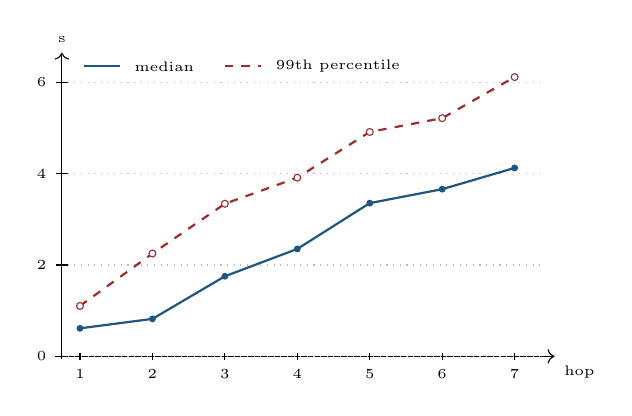
\begin{tikzpicture}[x=0.92cm,y=0.58cm,font=\scriptsize]
  \draw[->] (0.65,0) -- (7.55,0) node[below right,font=\tiny]{hop};
  \draw[->] (0.75,-0.05) -- (0.75,6.65) node[above,font=\tiny]{s};
  \foreach \x in {1,...,7} {
    \draw (\x,0.08) -- (\x,-0.08) node[below,font=\tiny]{\x};
  }
  \foreach \y in {0,2,4,6} {
    \draw (0.83,\y) -- (0.67,\y) node[left,font=\tiny]{\y};
    \draw[dotted,gray!55] (0.83,\y) -- (7.40,\y);
  }
  \draw[jbblue,thick]
    plot coordinates {(1,0.613) (2,0.820) (3,1.753) (4,2.352)
                      (5,3.355) (6,3.660) (7,4.125)};
  \foreach \x/\y in {1/0.613,2/0.820,3/1.753,4/2.352,5/3.355,6/3.660,7/4.125}
    \fill[jbblue] (\x,\y) circle (1.25pt);
  \draw[jbred,thick,dashed]
    plot coordinates {(1,1.104) (2,2.251) (3,3.341) (4,3.912)
                      (5,4.913) (6,5.215) (7,6.115)};
  \foreach \x/\y in {1/1.104,2/2.251,3/3.341,4/3.912,5/4.913,6/5.215,7/6.115}
    \draw[jbred,fill=white] (\x,\y) circle (1.25pt);
  \draw[jbblue,thick] (1.05,6.35) -- (1.55,6.35);
  \node[anchor=west,font=\tiny] at (1.62,6.35) {median};
  \draw[jbred,thick,dashed] (3.00,6.35) -- (3.50,6.35);
  \node[anchor=west,font=\tiny] at (3.57,6.35) {99th percentile};
\end{tikzpicture}
\caption{End-to-end projection latency by hop count for 200 paced posts in an eight-node chain with
a 1000 ms outbox drain interval. All 200 posts reached the final node.}
\label{fig:latency}
\end{figure}

An attempted parameter sweep was discarded. Repeating the same four-node, 500 ms-drain configuration
late in the sweep changed first-hop median latency by a factor of five. A fresh stack restored the
earlier value, indicating accumulated host contention rather than a parameter effect. We therefore
report one clean 200-sample configuration and do not infer scaling beyond it.

\section{Discussion and Limitations}

The evaluation supports mechanism feasibility, not national-shutdown availability. A one-host
container test reproduces route absence and source selection. It does not reproduce ISP routing
policy, deep packet inspection, heterogeneous clocks, packet loss, power failure, bridge coercion,
or independent operational decisions. A real two-provider experiment and repeated cut, blackhole,
loss, and failover trials are required before making field claims. The current crossing observation
has sample size one per condition.

The bridge is also a chokepoint. Signatures prevent undetected object modification, but they do not
force the bridge or any server to deliver, retain, or display content. Redundant bridges can reduce
availability risk, while introducing more observable endpoints and more peer-discovery surface.
First-contact trust remains vulnerable to eclipse attacks.

Security claims have similarly narrow boundaries. Author signatures establish authenticity and
integrity, not completeness or freshness. Stale-head suppression avoids one false alarm but is not a
substitute for consistency proofs. Origin-specific anti-abuse cannot be assumed at a malicious
server; receiving quotas bound its admitted rate. The system provides pseudonymity at the
application layer, not network anonymity. Timing, volume, key reuse, and writing style remain
linkable. Sixteen encoding vectors and conventional tests provide regression evidence, not formal
verification or exhaustive parser assurance.

The propagation run shares a host clock and storage process, which can suppress clock skew while
adding resource contention. The discarded sweep demonstrates that this confound is material. Raw
per-trial data, repeated configurations, randomized run order, and a control repeated throughout the
experiment are necessary for a stronger evaluation.

\section{Conclusion}

Federation across a partition depends on operational details that a global-reach design can leave
implicit. An endpointless node must be able to initiate both delivery directions. A multi-homed
relay must bind the correct source address, validate before relaying, and preserve capacity across
uplink pairs. Its scheduler must isolate peers because a blackholed route is expected during the
event the bridge is intended to survive. The prototype satisfied these properties in controlled
tests, delivered all 200 paced posts through a seven-hop path, and crossed a simulated exchange cut
through a verifying bridge. The evidence remains conditional on surviving domestic IP paths. Field
deployment across independent ISPs is the next test of the design, not a conclusion already
established by the container results.

\begin{thebibliography}{00}

\bibitem{bischof2023shutdowns}
Z. S. Bischof \emph{et al.}, ``Destination unreachable: Characterizing Internet outages and
shutdowns,'' in \emph{Proc. ACM SIGCOMM}, 2023, doi: 10.1145/3603269.3604883.

\bibitem{ooni2025bangladesh}
T. I. Raso, S. Afrin, M. A. Chowdhury, M. Xynou, and E. Yachmeneva, ``The longest silence:
Internet shutdowns during Bangladesh's 2024 uprising,'' OONI and Digitally Right, 2025. [Online].
Available: \url{https://ooni.org/post/2025-bangladesh-report/}

\bibitem{activitypub}
C. Lemmer-Webber, J. Tallon, E. Shepherd, A. Guy, and E. Prodromou, ``ActivityPub,'' W3C
Recommendation, Jan. 2018. [Online]. Available: \url{https://www.w3.org/TR/activitypub/}

\bibitem{wustrow2011telex}
E. Wustrow, S. Wolchok, I. Goldberg, and J. A. Halderman, ``Telex: Anticensorship in the network
infrastructure,'' in \emph{Proc. 20th USENIX Security Symp.}, 2011.

\bibitem{bocovich2024snowflake}
C. Bocovich, A. Breault, D. Fifield, Serene, and X. Wang, ``Snowflake, a censorship circumvention
system using temporary WebRTC proxies,'' in \emph{Proc. 33rd USENIX Security Symp.}, pp. 2635--2652,
2024.

\bibitem{raman2019mastodon}
A. Raman, S. Joglekar, E. De Cristofaro, N. Sastry, and G. Tyson, ``Challenges in the decentralised
web: The Mastodon case,'' in \emph{Proc. ACM Internet Measurement Conf.}, pp. 217--229, 2019, doi:
10.1145/3355369.3355572.

\bibitem{tarr2019ssb}
D. Tarr, E. Lavoie, A. Meyer, and C. Tschudin, ``Secure Scuttlebutt: An identity-centric protocol
for subjective and decentralized applications,'' in \emph{Proc. 6th ACM Conf. Information-Centric
Networking}, pp. 1--11, 2019, doi: 10.1145/3357150.3357396.

\bibitem{rfc9171}
S. Burleigh, K. Fall, and E. Birrane, ``Bundle protocol version 7,'' RFC 9171, Jan. 2022, doi:
10.17487/RFC9171.

\bibitem{rfc8445}
A. Keranen, C. Holmberg, and J. Rosenberg, ``Interactive connectivity establishment (ICE): A
protocol for network address translator traversal,'' RFC 8445, Jul. 2018, doi: 10.17487/RFC8445.

\bibitem{rfc8684}
A. Ford, C. Raiciu, M. Handley, O. Bonaventure, and C. Paasch, ``TCP extensions for multipath
operation with multiple addresses,'' RFC 8684, Mar. 2020, doi: 10.17487/RFC8684.

\bibitem{protobufcanonical}
Google, ``Proto serialization is not canonical,'' Protocol Buffers Documentation, 2024. [Online].
Available: \url{https://protobuf.dev/programming-guides/serialization-not-canonical/}

\bibitem{rfc9162}
B. Laurie, E. Messeri, and R. Stradling, ``Certificate transparency version 2.0,'' RFC 9162, Dec.
2021, doi: 10.17487/RFC9162.

\bibitem{bernstein2012ed25519}
D. J. Bernstein, N. Duif, T. Lange, P. Schwabe, and B.-Y. Yang, ``High-speed high-security
signatures,'' \emph{J. Cryptographic Engineering}, vol. 2, no. 2, pp. 77--89, 2012,
doi: 10.1007/s13389-012-0027-1.

\end{thebibliography}

\end{document}
